\chapter{经验分布函数、统计量及其分布}
\begin{introduction}
%   \item Intro to Prob\quad4.1 \quad 4.3 \quad 4.5 
  \item Prob $\&$ Stat\quad5.2,5.3
\end{introduction}
\section{引导问题:数据的价值2}
\begin{problem}
    既然总体是一个分布,我们能否基于来自这个总体的样本$x_{1},x_{2},\cdots,x_{n}$来猜测这个分布?
\end{problem}
\begin{note}
\vspace{3cm}
\end{note}
\section{经验分布函数}
\begin{definition}[经验分布函数]
    设$x_1,x_2,\cdots,x_n$是取自总体分布函数$F(x)$的样本,若将样本的观测值由小到大进行排列,记为$x_{(1)}\leq x_{(2)}\leq \cdots\leq x_{(n)}$,则称$x_{(1)}, x_{(2)}, \cdots, x_{(n)}$为\textbf{有序样本},用有序样本定义函数
    $$
    F_n(x) = \left\{
    \begin{aligned}
        &0, &\text{当$x<x_{(1)}$},\\
        & k/n, & \text{当$x_{(k)}\leq x<x_{(k+1)},k=1,2,\cdots,n-1$},\\
        &1, &\text{当$x\geq x_{(n)}$}.
    \end{aligned}
    \right.
    $$
    则$F_n(x)$是样本的\textbf{经验分布函数}。
\end{definition}
\begin{note}
    $F_n(x)$是一个分布函数。\\
    \vspace{5cm}
\end{note}

\begin{remark}
\begin{enumerate}
    \item 对固定的$x$,$F_n(x)$是样本中事件$\{x_i\leq x\}$发生的频率。 
    \item 当$n$固定时,$F_n(x)$是样本的函数,而样本是随机变量,所以$F_n(x)$也是一个随机变量。若对任意给定的实数$x$,定义
    $$
   I_i(x) = \left\{
   \begin{aligned}
       & 1, & x_i \leq x,\\
       & 0, & x_i > x.
   \end{aligned}
   \right.
    $$
    则经验分布函数的定义可以看出,$$
    F_n(x)= \frac{1}{n}\sum_{i=1}^n I_i(x).
    $$
    注意到$I_i(x)$是独立同分布的随机变量,其共同分布为$b(1,F(x))$.
    \item 由伯努利大数定律可知,只要$n$充分大,$F_n(x)$依概率收敛于$F(x)$.
\end{enumerate}    
\end{remark}

比较一下分布函数$F(x)$和经验分布函数$F_n(x)$的区别:
\begin{itemize}
  \item $F_{n}(x)$不是$F(x)$;
\item 但$F_{n}(x)$可代表$F(x)$;
\item $F_{n}(x)$可观测到,而$F(x)$不可观测到。
\end{itemize}


\begin{theorem}[格利文科定理]
设$x_{1},x_{2},\cdots,x_{n}$是取自总体分布函数为$F(x)$的样本,$F_{n}(x)$是其经验分布函数,当$n$充分大时,$F_{n}(x)$能充分逼近$F(x)$.
\end{theorem}

\begin{remark}
  格利文科定理保证了经典统计中一切统计推断都以样本为依据。  
\end{remark}
\section{统计量的定义}
\begin{definition}[统计量]
    设$x_1,x_2,\cdots,x_n$为取自某总体的样本,若样本函数
    $$
    T = T(x_1,x_2,\cdots,x_n)
    $$
    中不含任何未知参数,则称$T$为\textbf{统计量}。而统计量的分布称为\textbf{抽样分布}。
\end{definition}
\begin{remark}
\begin{enumerate}
    \item  统计量是可以通过样本直接计算而得的。
    \item 统计量是样本的函数,通常也作为随机变量来进行研究。
\end{enumerate}
\end{remark}
\begin{problem}
    既然统计量是一个随机变量,我们如何得到其分布呢?
\end{problem}
\begin{solution}
    其一,通过随机变量函数的分布的技术,我们可以得到统计量的精确分布;
    其二,在精确分布有困难时,我们也可以得到其近似分布。
\end{solution}

\newpage
\section{常见统计量:样本矩}
假定在样本$x_1,x_2,\cdots,x_n$中有$k$个不同的取值
$a_1,a_2,\cdots,a_k$。每一个样本$x_i$来自于一个均值为$\mu$和方差为$\sigma^2$分布的随机变量。

\begin{table}[ht]
\centering 
\begin{tabular}{c cccc}
\hline
数据 & $a_1$ & $a_2$ & $\cdots$ & $a_k$ \\ 
\hline
频数 & $m_1$ & $m_2$ & $\cdots$ & $m_k$ \\
\hline
频率 & $\frac{m_1}{n}$ & $\frac{m_2}{n}$ & $\cdots$ & $\frac{m_k}{n}$ \\
\hline
\end{tabular}
\end{table}



\begin{remark}
    $\sum_{i=1}^{k} m_{i}=n ,\sum_{i=1}^{k} a_{i} m_{i}=\sum_{i=1}^{n} x_{i}$。
\end{remark}

因为$F_n(x)$是一个某个随机变量的分布函数,假定该随机变量为$X$,所以,
\begin{eqnarray*}
E_{F_{n}}(X) &=&\sum_{i=1}^{k} a_{i} \cdot \frac{m_{i}}{n}=\frac{1}{n} \sum_{i=1}^{k} a_{i} m_{i}=\frac{1}{n} \sum_{i=1}^{n} x_{i} \\
E_{F_{n}}\left(X^{l}\right) &=&\sum_{i=1}^{k} a_{i}^{l} \frac{m_{i}}{n}=\frac{1}{n} \sum_{i=1}^{k} a_{i}^{l} m_{i}=\frac{1}{n} \sum_{i=1}^{n} x_{i}^{l} 
\end{eqnarray*}
\begin{eqnarray*}
\text{Var}_{F_{n}}(X) &=&\sum_{i=1}^{k}\left(a_{i}-E_{F_{n}}(X)\right)^{2} \cdot \frac{m_{i}}{n} \\
&=&\sum_{i=1}^{k}\left(a_{i}-\bar{x}\right)^{2} \cdot \frac{m_{i}}{n} \\
&=&\frac{1}{n} \sum_{i=1}^{k}\left(a_{i}-\bar{x}\right)^{2} \cdot m_{i} \\
&=&\frac{1}{n} \sum_{i=1}^{n}\left(x_{i}-\bar{x}\right)^{2} 
\end{eqnarray*}
\begin{remark}
    我们通常记$\bar{x} = \frac{1}{n}\sum_{i=1}^{n} x_{i} $,而$s_{n}^2 = \frac{1}{n} \sum_{i=1}^{n}\left(x_{i}-\bar{x}\right)^{2} $。
\end{remark}

\begin{definition}
    设$x_1,x_2,\cdots,x_n$是样本,$k$为正整数,则统计量
    $$
    a_k = \frac{1}{n} \sum_{i=1}^n x_i^k
    $$
    称为样本$k$阶原点矩;统计量
    $$
    b_k = \frac{1}{n} \sum_{i=1}^n (x_i-\bar{x})^k
    $$
    称为样本$k$阶中心矩。
\end{definition}
\begin{remark}
    样本一阶原点矩是样本均值;样本二阶中心矩是样本方差。
\end{remark}

\subsection{样本均值}
样本均值$\bar{x}$是最简单的统计量。首先考察其期望和方差。我们可以证明
\begin{eqnarray*}
    E(\bar{x}) &=& E\left( \frac{1}{n}\sum_{i=1}^{n} x_{i}  \right) = \frac{1}{n}\sum_{i=1}^{n} E(x_{i}) = \mu \\
    \text{Var}(\bar{x}) &=& \text{Var} \left( \frac{1}{n}\sum_{i=1}^{n} x_{i}  \right) = \frac{1}{n^2}\sum_{i=1}^{n} \text{Var}(x_{i})  = \frac{\sigma^2}{n}.
\end{eqnarray*}

其次,我们考虑$\bar{x}$的分布。
\begin{enumerate}
    \item 精确分布:如果$x_{1}, x_{2}, \ldots, x_{n}$均来自正态分布$N\left(\mu, \sigma^{2}\right) $,那么$\bar{x}$的分布是$N(\mu,\sigma^2/n)$。
    \item 近似分布1(渐近分布):如果$x_{1}, x_{2}, \ldots, x_{n}$均来自未知分布$\Pi\left(\mu, \sigma^{2}\right) $,那么,根据CTL,
    $$
    \frac{\bar{x}-E(\bar{x})}{\sqrt{{\text{Var}}(\bar{x})}} \stackrel{L}{\longrightarrow} N(0,1).
    $$
    \item 近似分布2(蒙特卡洛分布):如果$x_{1},x_{2},\cdots,x_{5}$来自于指数分布$Exp(1/5)$,那么$\bar{x} = \frac{1}{5}\sum_{i=1}^5x_i$的蒙特卡洛分布应如图\ref{fig:Lect16_MC_dist_EXP}所示。图中直方图刻画的是$\bar{x}$的蒙特卡洛分布,而红线表示的是其真实的密度函数。
\begin{figure}[ht]
    \centering
    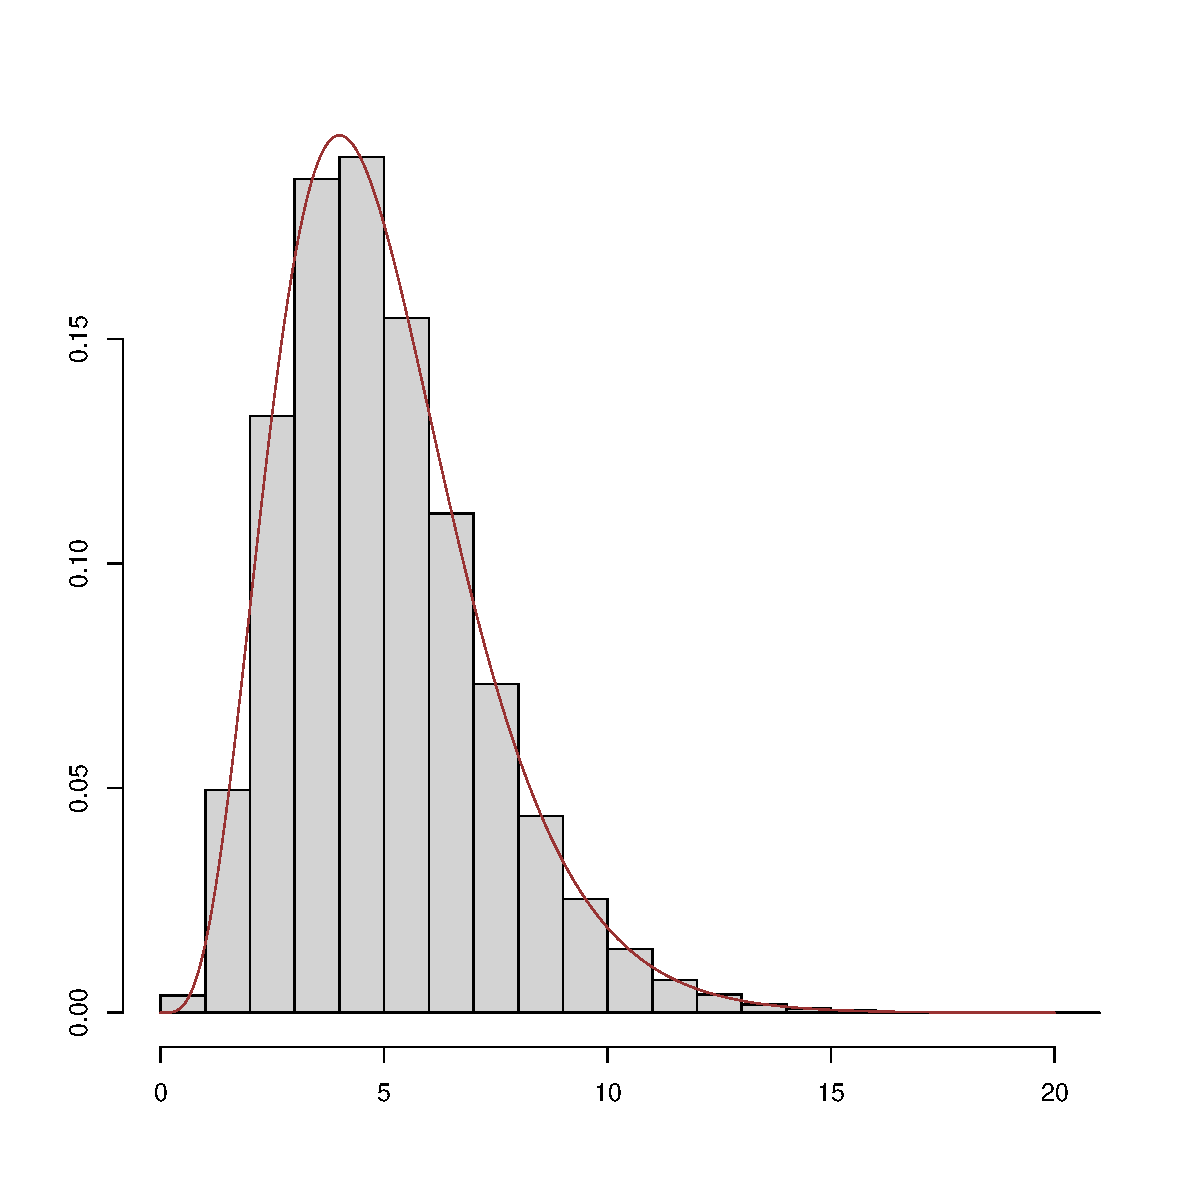
\includegraphics[width=0.5\linewidth]{image/Lect16_MC_dist_EXP.pdf}
    \caption{蒙特卡洛分布}
    \label{fig:Lect16_MC_dist_EXP}
\end{figure}

在实现蒙特卡洛分布时,只需要进行以下三步:
\begin{enumerate}
    \item 从指数分布$Exp(1/5)$产生$5$个随机数:$x_1^{m},x_2^{m},,\cdots,x_5^{m}$;
    \item 计算$\bar{x}^{m} = \frac{1}{5}\sum_{i=1}^5x_i^{m};$
    \item 重复前面两步$M$次。
\end{enumerate}
由此可以得到$M$个样本均值的取值,来得到其经验分布函数。
\begin{problem}
    如何保留蒙特卡洛分布的信息?
\end{problem}

\begin{problem}
    请问$\bar{x}$的真实分布是什么?
\end{problem}
\end{enumerate}

    
\subsection{样本方差和样本标准差}
样本方差$s_{n}^2$也是一种常用的统计量。为了考虑$s_{n}^2$的期望,我们可以计算偏差平方和$\sum_{i=1}^{n}\left(x_{i}-\bar{x}\right)^{2}$的期望,即
\begin{eqnarray*}
E\left( \sum_{i=1}^{n}\left(x_{i}-\bar{x}\right)^{2}\right) 
&=& E\left(\sum_{i=1}^{n}\left(x_{i}^{2}-2 x_{i} \bar{x}+\bar{x}^{2}\right)\right) \\
&=& E\left(\sum_{i=1}^{n} x_{i}^{2}-2 n \bar{x}^{2}+n \bar{x}^{2}\right) \\
&=& E\left(\sum_{i=1}^{n} x_{i}^{2}-n \bar{x}^{2}\right) \\
&=&\left(\sum_{i=1}^{n} E\left(x_{i}^{2}\right)-n E\left(\bar{x}^{2}\right)\right) \\
&=&\left[\sum_{i=1}^{n}\left(\text{Var}\left(x_{i}\right)+E^2\left(x_{i}\right)\right)-n\left(E^{2}(\bar{x})+\text{Var}(\bar{x})\right)\right] \\
&=& \cdot\left(n \cdot\left(\sigma^{2}+\mu^{2}\right)-n\left(\mu^{2}+\frac{\sigma^{2}}{n}\right)\right) \\
&=&(n-1) \sigma^{2}
\end{eqnarray*}
因此,我们发现$E(s_n^2) = (n-1)\sigma^2/n \neq \sigma^2$。在实际中,我们常采用$$
\frac{1}{n-1} \sum_{i=1}^{n}\left(x_{i}-\bar{x}\right)^{2}
$$
作为样本方差。而定义样本标准差为$s = \sqrt{s^2}$。
\subsection{样本偏度和样本峰度(选修)}
\begin{definition}
    设$x_1,x_2,\cdots,x_n$是样本,则称统计量
    $$
    \hat{\beta}_s = \frac{b_3}{b_2^{3/2}}
    $$
    为样本偏度;
    称统计量
    $$
    \hat{\beta}_k = \frac{b_4}{b_2^2} - 3
    $$
    为样本峰度。
\end{definition}
\newpage
\section{常见统计量:次序统计量}
\begin{example}
    我们共有$n$个学生参加本学期的期中考试,记为$x_1,x_2,\cdots,x_{n}$。常常会对学生的考试成绩进行排名,学生的考试成绩可以按从小到大进行排序,于是可以得到一组有序样本$x_{(1)}\leq x_{(2)}\leq \cdots \leq x_{(n)}$。我们记$y_i = x_{(i)}$。易知,$y_1,y_2,\cdots,y_{n}$既不独立也不同分布。
\end{example}
\begin{definition}
    设$x_1,x_2,\cdots,x_n$是来自于总体$X$的样本,$x_{(i)}$称为样本的第$i$个次序统计量,它表示将样本观测值从小到大排序后得到的第$i$个观测值,其中$x_{(1)}=\min\{x_1,x_2,\cdots,x_n\}$称为该样本的最小次序统计量,$x_{(n)}=\max\{x_1,x_2,\cdots,x_n\}$称为该样本的最大次序统计量,$(x_{(1)},x_{(2)},\cdots,x_{(n)})$称为该样本的次序统计量。
\end{definition}

\begin{problem}
\begin{enumerate}
    \item 如何求$x_{(k)}$的分布?
    \item 如何求$x_{(n)} - x_{(1)}$的分布?
\end{enumerate}
\end{problem}



\begin{theorem}
设总体$X$的密度函数为$p(x)$,分布函数为$F(x)$,$x_1,x_2,\cdots,x_n$为样本,则第$k$个次序统计量$x_{(k)}$的密度函数为
$$
p_k(x) = \frac{n!}{(k-1)!(n-k)!} (F(x))^{k-1} (1-F(x))^{n-k} p(x).
$$
\end{theorem}
以下给出两种证明方法。
\begin{proof}
    因为我们需要将$x_{(k)}$看成一个随机变量,所以记$X_{(k)}$为第$k$个次序统计量。
    首先考虑$X_{(k)}$的分布函数$F_{k}(x) = P(X_{(k)}\leq x)$。注意到事件
    \begin{eqnarray*}
        \left\{
    X_{(k)} \leq x
    \right\} &\Leftrightarrow& \left\{
    x_1,x_2,\cdots,x_n\text{中至少有$k$个}\leq x
    \right\} \\
    &\Leftrightarrow& \cup_{j=k}^{n} \left\{
    x_1,x_2,\cdots,x_n\text{中恰好有$j$个}\leq x
    \right\}
    \end{eqnarray*}
    
    所以,
    \begin{eqnarray*}
        F_k(x) 
        &=& \sum_{j=k}^n P\left( x_1,x_2,\cdots,x_n\text{中恰好有$j$个}\leq x \right)\\
        &=&\sum_{j=k}^n  C_{n}^j (F(x))^{j} (1-F(x))^{n-j}
    \end{eqnarray*}
    根据引理2.1,我们可知
    $$
     F_k(x) = \int_{0}^{F(x)} \frac{n!}{(k-1)!(n-k)!} x^{k-1}(1-x)^{n-k}\text{d}x.
    $$
    于是,定理得证。
\end{proof}

\begin{lemma}
    对于$0<p<1$,有
    $$
    \sum_{j=k}^n C_n^j p^j(1-p)^{n-j} = \int_{0}^p \frac{n!}{(k-1)!(n-k)!} x^{k-1}(1-x)^{n-k}\text{d}x
    $$
\end{lemma}
\begin{proof}
    令$$
    g(p) =  \sum_{j=k}^n C_n^j p^j(1-p)^{n-j}.
    $$
    于是,关于$g(p)$对$p$求导,即
    \begin{eqnarray*}
        \frac{\partial }{\partial p} g(p) &=&  \frac{\partial }{\partial p}\left( \sum_{j=k}^n C_n^j p^j(1-p)^{n-j}\right)\\
        &=& \sum_{j=k}^n \left(\frac{\partial }{\partial p}  p^j(1-p)^{n-j}\right)
    \end{eqnarray*}
    注意到,第$k$项为$$
C_n^k\left(k p^{k-1}(1-p)^{n-k}-(n-k)p^{k}(1-p)^{n-k-1}\right),$$
而第$k+1$项为
$$
C_n^{k+1}\left((k+1) p^{k}(1-p)^{n-k-1}-(n-k-1) p^{k+1}(1-p)^{n-k-2}\right).$$
同时,
$$
C_n^k p^{k}(n-k)(1-p)^{n-k-1} = C_n^{k+1}(k+1) p^{k}(1-p)^{n-k-1}.
$$
所以,进行前后消除,我们有
$$\frac{\partial}{\partial p} g(p)=\frac{n !}{(k-1) !(n-k) !} p^{k-1}(1-p)^{n-k}.$$
我们可以验证其初始值相等即可。
\end{proof}

\begin{proof}
    对任意的实数$x$,考虑次序统计两个$x_{(k)}$取值落在小区间$(x,x+\Delta x]$内这一事件,它等价于“样本量$n$的样本中有1个观测值落在$(x,x+\Delta x]$之间(多于一个观测值落在区间)$(x,x+\Delta x]$的概率是$\Delta x$的高阶无穷小量,后同),而有$k-1$个观测值小于等于$x$,有$n-k$个观测值大于$x+\Delta x$”。

    样本的每一个分量小于等于$x$的概率是$F(x)$,落入区间$(x,x+\Delta x]$的概率为$F(x+\Delta x)-F(x)$,大于$x+\Delta x$的概率为$1-F(x+\Delta x)$,而将$n$个分量分成这样的三组,总的分法有$\frac{n!}{(k-1)!11!(n-k)!}$种。于是,若以$F_k(x)$记$x_{(k)}$的分布函数,则由多项式分布可得
    $$
    F_k(x+\Delta x) - F_k(x) \approx \frac{n!}{(k-1)!11!(n-k)!} (F(x))^{k-1} (F(x+\Delta x)-F(x))(1-F(x+\Delta x))^{n-k},
    $$
    两边除以$\Delta x$,并令$\Delta x \rightarrow 0$,即有
    \begin{eqnarray*}
        p_k(x) &=& \lim_{\Delta x \rightarrow 0} \frac{F_k(x+\Delta x) - F_k(x)}{\Delta x}\\
        &=& \frac{n!}{(k-1)!1!(n-k)!} (F(x))^{k-1} p(x)(1-F(x+\Delta x))^{n-k}
    \end{eqnarray*}
    其中$p_k(x)$的非零区间与总体的非零区间相同。
\end{proof}
    
 
\begin{theorem}
    对于统计量$(x_{(i)},x_{(j)})(i<j)$得联合分布密度函数为
    \begin{eqnarray*}
        p_{ij}(y,z) &=& \frac{n!}{(i-1)!(j-i-1)!(n-j)!} \\
        &&(F(y))^{i-1} (F(z)-F(y))^{j-i-1}(1-F(z))^{n-j}p(y)p(z), y\leq z.
    \end{eqnarray*}

\end{theorem}
\begin{proof}
对增量$\Delta y, \Delta z$以及$y<z$,事件$\{x_{(i)} \in (y,y+\Delta y], x_{(j)} \in  (z , z+\Delta z]\}$可以表述为“样本量为$n$的样本$x_1,x_2,\cdots,x_n$中有$i-1$个观测值小于等于$y$,一个落入区间$(y,y+\Delta y]$,$j-i-1$个落入区间$(y+\Delta y, z]$, 一个落入区间$(z,z+\Delta z]$,而余下$n-j$个大于$z+\Delta z$”。
于是由多项式分布可得
\begin{eqnarray*}
    &&P(x_{(i)}\in (y,y+\Delta y] , x_{(j)}\in (z,z+\Delta z]) \\
    &\approx& \frac{n!}{(i-1)!1!(j-i-1)!1!(n-j)!}(F(y))^{i-1} p(y)\Delta y\\
    &&(F(z) - F(y+\Delta y))^{j-i-1} p(z)\Delta z (1-F(z+\Delta z))^{n-j}, 
\end{eqnarray*}
考虑到$F(x)$的连续性,当$\Delta y \rightarrow 0, \Delta z \rightarrow 0$时,有$F(y+\Delta y) \rightarrow F(y),F(z+\Delta z) \rightarrow F(z) $,于是
\begin{eqnarray*}
    p_{ij}(y,z) &=& \lim_{\Delta y \rightarrow 0,\Delta z \rightarrow 0} \frac{P(x_{(i)}\in (y,y+\Delta y] , x_{(j)}\in (z,z+\Delta z])}{\Delta y \cdot \Delta z}\\
    &=& \frac{n!}{(i-1)!1!(j-i-1)!1!(n-j)!}(F(y))^{i-1} p(y) \\
    &&(F(z) - F(y+\Delta y))^{j-i-1} p(z)(1-F(z+\Delta z))^{n-j}
\end{eqnarray*}
\end{proof}

\begin{example}
    设总体分布为$U(0,1)$,$x_1,x_2,\cdots,x_n$为其样本,则
\begin{enumerate}
    \item $x_{(k)}$的分布是$Be(k,n-k+1)$.

    因为$x_i$的分布函数为$$F(x) = 
    \left\{\begin{aligned}
    &0, & x\leq 0\\
     &   x, &0<x<1\\
     & 1 , & x\geq 1.\\
    \end{aligned}\right.
    $$
    所以,$x_{(k)}$的密度函数为
    \begin{eqnarray*}
        p_k(x) &=& \frac{n!}{(k-1)!(n-k)!} x^{k-1}(1-x)^{n-k} \\
        &=& \frac{\Gamma(n+1)}{\Gamma(k)\Gamma(n-k+1)} x^{k-1}(1-x)^{(n-k+1)-1}, 0<x<1.
    \end{eqnarray*}
    \item $(x_{(k)},x_{(s)})$的联合密度函数为
    $$
    p_{k,s}(x,y)=\frac{n!}{(k-1)!(s-k-1)!(n-s)!} x^{k-1}(y-x)^{s-k-1}(1-y)^{n-s}, 0\leq x\leq y\leq 1.
    $$
    \item 若$Y=x_{(s)}-x_{(k)}$。令$U=x_{(k)}$。则$Y$的密度函数为
    \begin{eqnarray*}
p_{Y}(y)&=&\int_{0}^{1-y} p(y, u) \text{d} u\\
&=&\int_{0}^{1-y} \frac{n !}{(k-1) !(s-k-1) !(n-s) !} u^{k-1} y^{s-k-1}(1-u-y)^{n-s} \text{d} u\\
&\overset{u=(1-y)v}{=}&\frac{n !}{(k-1) !(s-k-1) !(n-s) !}\\
&&\cdot\int_{0}^{1} (1-y)^{k-1} v^{k-1} y^{s-k-1}(1-y)^{n-s}(1-v)^{n-s}(1-y) \text{d} v\\
&=&y^{s-k-1}(1-y)^{n-s+k} \int_{0}^{1} \frac{n !}{(k-1) !(s-k-1) !(n-s) !} v^{k-1}(1-v)^{n-s} \text{d} v\\
&=& y^{s-k-1}(1-y)^{n-s+k} \cdot \frac{n!}{{(k-1)!}(s-k-1)!{(n-s)!}}\cdot \frac{{(k-1)!}{(n-s)!}}{(n+k-s)!}\\
&& \int_{0}^{1} \frac{\Gamma(n+k-s+1)}{\Gamma(k) \Gamma(n-s+1)} v^{k-1}(1-v)^{(n-s+1)-1} \text{d} v\\
&=&\frac{\Gamma(n+1)}{\Gamma(s-k) \Gamma(n-s+k+1)} y^{(s-k)-1}(1-y)^{(n-s+k+1)-1}
    \end{eqnarray*}
   因此,$Y$的分布是$Be(s-k,n-s+k+1)$。
\end{enumerate}    
\end{example}

\begin{remark}
    \begin{enumerate}
       \item 均匀分布的次序统计量是贝塔分布的来源之一。
        \item 经验分布函数是次序统计量的函数,即
         $$F_{n}(x)=\frac{1}{n} \sum_{i=1}^{n} I_{\left\{x_{i} \leq x\right\}}=\frac{1}{n} \sum_{i=1}^{n} I\left\{X_{(i)} \leq x\right\}.$$
         \item 样本分位数也是基于次序统计量而定义。
    \end{enumerate}
\end{remark}

\subsection{样本分位数}
\begin{definition}
    $m_{0.5}$定义如下:
    $$
    m_{0.5} = \left\{\begin{aligned}
        & x_{\left(\frac{n+1}{2}\right)} & n\text{为奇数}, \\
&\frac{1}{2}\left(x_{\left(\frac{n}{2}\right)}+x_{\left(\frac{n}{2}+1\right)}\right) & n\text{为偶数}.
    \end{aligned}
    \right.
    $$
    称$m_{0.5}$为中位数。
\end{definition}

\begin{definition}
    $m_{p}$定义如下:
    $$
    m_{p} = \left\{\begin{aligned}
        & x_{\left([np+1]\right)} & \text{若$np$不为整数}, \\
&\frac{1}{2}\left(x_{\left([np]\right)}+x_{\left( [np+1]\right)}\right) & \text{若$np$为整数}.
    \end{aligned}
    \right.
    $$
    称$m_{p}$为样本$p$分位数。
\end{definition}

对于样本分位数,我们也有相应的渐近分布,如下定理,供学生进行选修。
\begin{theorem}
    设总体密度函数为$p(x)$,$x_p$为其$p$分位数,$p(x)$在$x_p$处连续且$p(x_p)>0$,则当$n\rightarrow \infty$时,样本$p$分位数$m_p$的渐近分布为
    $$
    m_p \overset{\cdot}{\sim } N\left(x_p, \frac{p(1-p)}{np^2(x_p)}\right).
    $$
    特别地,对于样本中位数,当$n\rightarrow \infty$时近似地有
    $$
    m_{0.5} \overset{\cdot}{\sim } N\left(x_{0.5}, \frac{1}{4np^2(x_{0.5})}\right).
    $$
\end{theorem}






% 推广:考虑$(X(k), X(s))$的联合密度函数
% \begin{figure}[H]
%   \centering
%   \includegraphics[width=0.6\textwidth]{image/15.2.jpg}
% \end{figure}

% $p_{(k,s)}(x,y)$$=\left(\begin{array}{l}
% n \\
% k-1
% \end{array}\right)(F(x))^{k-1}\left(\begin{array}{c}
% n-(k-1) \\
% 1
% \end{array}\right) p(x) \left(\begin{array}{c}
% n-k \\
% s-k-1
% \end{array}\right)(F(y)-F(x))^{s-k-1}\left(\begin{array}{c}
% n-(s-1) \\
% 1
% \end{array}\right) p(y) \cdot(1-F(y))^{n-s}$

% 补充:多元组合数 
% \begin{figure}[H]
%   \centering
%   \includegraphics[width=0.6\textwidth]{image/15.3.jpg}
% \end{figure}   

% \begin{problem}
%         有多少种方法?
%         \end{problem}

% $$\begin{aligned}
% &\left(\begin{array}{c}
% n \\
% k_{1}
% \end{array}\right)\left(\begin{array}{c}
% n-k_{1} \\
% k_{2}
% \end{array}\right)\left(\begin{array}{c}
% n-k_{1}-k_{2} \\
% k_{3}
% \end{array}\right) \\
% =& \frac{n !}{k_{1} !\left(n-k_{1}\right) !} \frac{\left(n-k_{1}\right) !}{k_{2} !\left(n-k_{1}-k_{2}\right) !} \cdot \frac{\left(n-k_{1}-k_{2}\right) !}{k_{3} !\left(n-k_{1}-k_{2}-k_{3}\right) !} \\
% =& \frac{n !}{k_{1} ! k_{2} ! k_{3} !}
% \end{aligned}$$

% 那么 $$\begin{aligned}
% & P(k, g)(x, y) \\
% =& \frac{n !}{(k-1) !(s-k-1) !(n-s) !}(F(x))^{k-1}(F(y)-F(x))^{s-k-1}(1- F(s))^{n-s} p(x) \cdot p(y)
% \end{aligned}$$

\section{习题}
\begin{enumerate}
    \item 设$x_1,x_2,x_n$和$y_1,y_2,\cdots,y_n$是两组样本观测值,且关系如下:
$$
y_i = a x_i + b, i=1,2,\cdots,n
$$
其中,$a$和$b$为非零常数。试求:
\begin{enumerate}
    \item 样本均值$\bar{x}$和$\bar{y}$间的关系;
\item 样本方差$s_x^2$和$s_y^2$间的关系。
\end{enumerate}

\item 设总体$X$的$3$阶矩存在,若$x_1,x_2,\cdots,x_n$是取自该总体的简单随机样本,$\bar{x}$为样本均值,$s^2$为样本方差,试证:
$$
\text{Cov}(\bar{x},s^2) = \frac{\nu_3}{n},
$$
其中$\nu_3 = E(x-E(x))^3$。

\item 设$\bar{x}_1$和$\bar{x}_2$是从同一正态总体$N(\mu,\sigma^2)$独立抽取的容量相同的两个样本均值。试确定样本容量$n$,使得两样本均值的差超过$\sigma$的概率不超过$0.01$。

\item 从指数总体$Exp(1/\theta)$抽取了$40$个样品,试求$\bar{x}$的渐近分布。

\item  设总体$X$的分布函数$F(x)$是连续的,$x_{(1)},x_{(2)},\cdots,x_{(n)}$为取自此总体的次序统计量,设$\eta_i = F(x_{(i)})$,试证:
\begin{enumerate}
    \item $\eta_1 \leq \eta_2 \leq \cdots \leq \eta_n$,$\eta_i$是来自均匀分布$U(0,1)$总体的次序统计量;
\item $E(\eta_i) = \frac{i}{n+1}$,$\text{Var}(\eta_i) = \frac{i(n+1-i)}{(n+1)^2(n+2)}, 1\leq i\leq n$;
\item $\eta_i$和$\eta_j$的协方差矩阵为
$$
\begin{pmatrix}
\frac{a_1(1-a_1)}{n+2} & \frac{a_1(1-a_2)}{n+2}\\
\frac{a_1(1-a_2)}{n+2} & \frac{a_2(1-a_2)}{n+2}
\end{pmatrix}
$$
其中,$a_1 = \frac{i}{n+1},a_2  = \frac{j}{n+1}$.
\end{enumerate}
\end{enumerate}
